
\documentclass{acm_proc_article-sp}
\usepackage{graphicx}
\usepackage{caption}
\usepackage[english]{babel}
\usepackage{subcaption}
\usepackage{gensymb}
\begin{document}

\title{3D interaction in virtual environments: Jet Fighter}

%
% Authors
%
\numberofauthors{4} 
\author{
    \alignauthor Jens Brulmans\\
    \affaddr{Universiteit Hasselt}\\
    \affaddr{Agoralaan - Gebouw D}\\
    \affaddr{Diepenbeek, Belgie}\\
    \affaddr{jens.brulmans@}\\
    \affaddr{student.uhasselt.be}\\
    \alignauthor Ben Clerix\\
    \affaddr{Universiteit Hasselt}\\
    \affaddr{Agoralaan - Gebouw D}\\
    \affaddr{Diepenbeek, Belgie}\\
    \affaddr{ben.clerix@}\\
    \affaddr{student.uhasselt.be}\\
    \alignauthor Cedric Lodts\\
    \affaddr{Universiteit Hasselt}\\
    \affaddr{Agoralaan - Gebouw D}\\
    \affaddr{Diepenbeek, Belgie}\\
    \affaddr{cedric.lodts@}\\
    \affaddr{student.uhasselt.be}\\
    \and
    \alignauthor Bram Meerten\\
    \affaddr{Universiteit Hasselt}\\
    \affaddr{Agoralaan - Gebouw D}\\
    \affaddr{Diepenbeek, Belgie}\\
    \affaddr{bram.meerten@}\\
    \affaddr{student.uhasselt.be}\\
}

\date{16 December 2014}

\maketitle
\begin{abstract}
In this paper we describe different ways for interaction in a 3D-environment with a Kinect through a Unity game. We use a 3D jet-fighter arcade game as a setting for a small test environment and develop interactions such as for shooting enemy planes.
These interactions have to be developed in a way to get as much user comfort as possible (and as less awkward body movement as possible) for the user while still being easy to use. We developed and described different ways for navigation, manipulation and selection in this paper.
We conclude that mapping all the different interactions for navigation, manipulation and selection for a single person using the Kinect without using any other hardware can be a difficult process if you want to keep usability in mind.
\end{abstract}

\keywords{Kinect, 3D interaction, virtual environments, HCI, gestures, Unity}

\section{Introduction}
Navigation, manipulation and selection in a virtual \newline 3D-environment is a big research-topic. We will describe a way to implement these interaction methods in a jet fighter arcade-game setting that we built with the Unity engine using a Kinect to track the user's gestures. In this game, the player controls a jet fighter and has to complete certain objectives. We implemented four different ways to navigate the jet fighter. We tested these techniques out ourselves and by a few other fellow students that were not affiliated with this research. In section \ref{sec:Applicationdomain} we elaborate on the application domain. The challenges we want to tackle are described in section \ref{sec:Challenges}. Section \ref{sec:Interactiontechniques} lists the different interaction techniques for navigation, manipulation and selection.
\begin{figure}[ht]
\centering
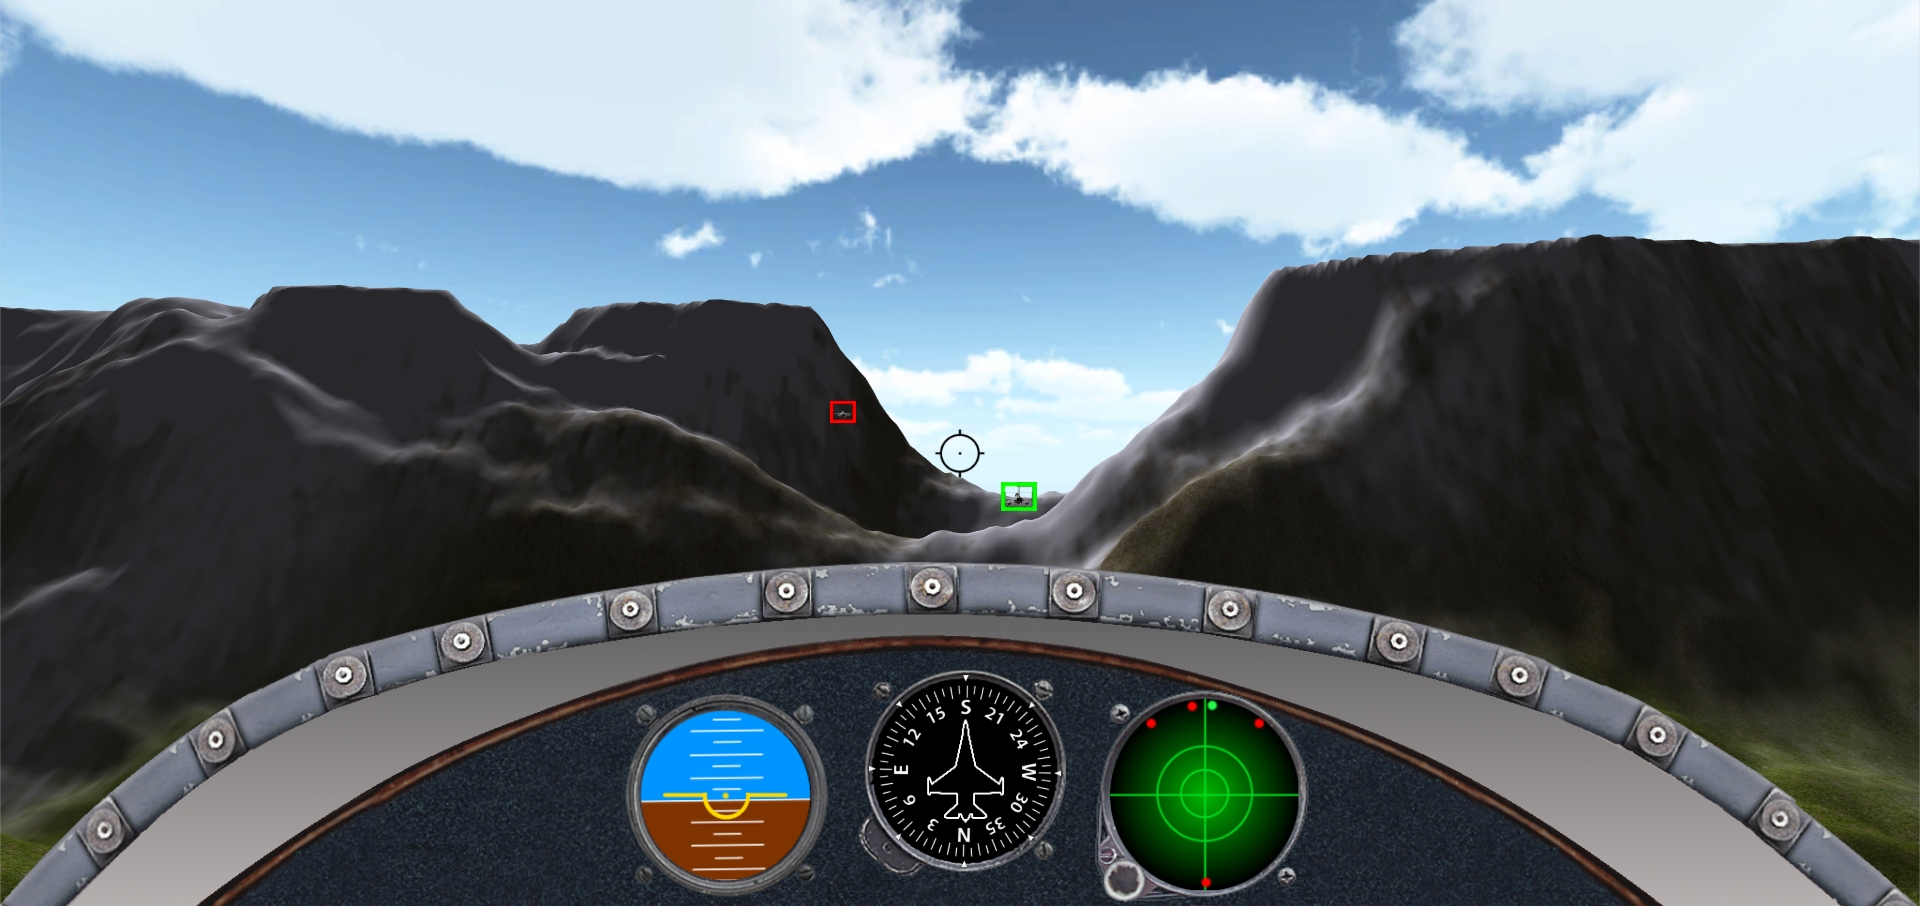
\includegraphics[width=0.5\textwidth ,keepaspectratio=true]{./img/overviewScreen.jpg}
\caption{Overview screen of the application}
\label{overview}
\end{figure}

\section {Application domain}\label{sec:Applicationdomain}
We aim to research different interaction techniques for navigation, manipulation and selection in a virtual 3D-environment. To test these interaction methods, we developed a first-person jet-fighter game by using the Unity engine. In this game, the player controls a jet fighter and is given different objectives to complete. The player can get an objective to fly through hoops in the air or to shoot down a targeted enemy aircraft. 
Using the Kinect, the player will have to control a jet fighter at high velocity and be able to aim, shoot and control the speed of the aircraft all at the same time.
We developed different navigation methods and by trying them ourselves, determined which one had the most user comfort in our opinion. The jet fighter is controlled with a manual navigation and target selection technique. There is also an  option to turn on an auto-pilot which will cause the jet fighter to follow a targeted enemy plane. The player also has the ability switch between a machine gun that fires straight forward and a homing missile that will follow the targeted enemy.

\section {Challenges}\label{sec:Challenges}
The main challenge is mapping all the different actions onto distinguishable gestures for a single player while keeping user task performance, ease of use and user comfort in mind. Ideally the player could navigate the plane and simultaneously select and shoot enemy planes. However this requires the user to perform at least three gestures at the same time, which is hard because the gestures will interfere with each other and may cause the player to be in an uncomfortable situation. 

Another challenge is selecting target enemy planes. There can be multiple planes and they can be rather small. This means we have to find a way to easily select enemies and confirm the selection. Confirming the selection is necessary so the player does not accidentally select a wrong target.

\section {Hardware}\label{sec:hardware}
For the hardware to control the plane, we chose the Kinect as a way to detect body-movement and gestures. During the development of the application, we also noticed a foot pedal was easier to use than a confirmation gesture.
\subsection{Kinect}
The XBOX 360 Kinect is used for getting the user's body position and movement. We track this information and use it to control the plane's speed, rotation and actions.

\subsection{Pedal}
After selecting a plane there still needs to be a way to confirm the selection. At first a gesture was used for this but later on we decided to try a pedal for this and kept this as an easy way to confirm the selection with the push of a button.

\section {Interaction techniques}\label{sec:Interactiontechniques}
The game needs to support six different actions that because of the Kinect movement-control are all constrained by the ``flexibility'' of the user (see table \ref{tblActions}). Another constraint is mapping all of these different actions on the limbs of a user.

\begin{table}
\centering
\caption{In-game actions}
\begin{tabular}{|l|} \hline
\bf{Action} \\ \hline
Navigate left/right\\ \hline
Navigate up/down\\ \hline
Select target \\ \hline
Shoot missile \\ \hline
Shoot machine gun \\ \hline
Change speed \\ \hline
\end{tabular}
\label{tblActions}
\end{table}

\subsection{Navigation}
The navigation can be an active solution where the user has to control everything manually or a passive solution where the user is helped by the system by things like an auto-pilot \cite{bookactivepassive}.

Our navigation technique is a virtual travel technique\cite{bookactivepassive}. This means that the user's body remains stationary even though the virtual viewpoint moves. A physical travel technique, the counterpart of a virtual travel technique, in which a movement of the user's body translates to a movement in the virtual viewpoint. For example, if the user turns around the viewpoint also turns around, this is not the case in our application.

We have tried four different approaches for navigation (Figure \ref{naviagationapproaches}).
All of them are an active or hybrid technique and all of them use a torso-directed steering technique \cite{booktorso}.

The first navigation technique uses the angle of the user's body to tilt the aircraft.
The further the user leans in a certain direction, the faster the plane will turn in that direction.
When the user stands up straight, the plane will automatically balances back to go straight forward.
The hands could still be used for selection actions.
A disadvantage however is that the gestures for manipulation will inevitably interfere with the navigation gesture because they occlude the view of the Kinect. A second disadvantage is that the human body is not made to lean backwards by more than a certain degrees, therefore elevating the plane by leaning backwords will be hard for the user.

For the second navigation technique we map the angle of the user's body directly on the plane (position control instead of force control \cite{bookpositionforcecontrol}).
e.g. If the user leans 10\degree left, the plane will tilt 10\degree left. The downside to this was that this eliminates the option for the player to turn 360\degree. It does mean that the arms could still be used for selection actions.

The third navigation technique uses the left arm to make the plane point up or down. The user has to lean left or right to make the plane tilt left and right. This means that only the right arm was left for manipulation actions.
Because we couldn't get all the actions mapped, we discarded this technique and carried on with a new one.
A disadvantage is that is difficult to simultaneously navigate with one arm and manipulate with the other because the human body cannot multitask effectively.
   
The fourth navigation technique we implemented is the one we chose for the final result. It uses the first technique for manual steering but it adds in the option to turn on an auto-pilot by keeping your left arm next to your body. The auto-pilot steers the plane directly in the direction of a targeted enemy aircraft (a target-based technique \cite{booktargetbased}). An enemy aircraft will always be selected automatically. If there are multiple possible targets, the player can select which enemy he/she wants to target by moving the right arm in the direction of the target he/she wants to select.
%Maybe remove the disadvantages of each technique and move them to the evaluation or testing section


\begin{figure}[ht]
\centering
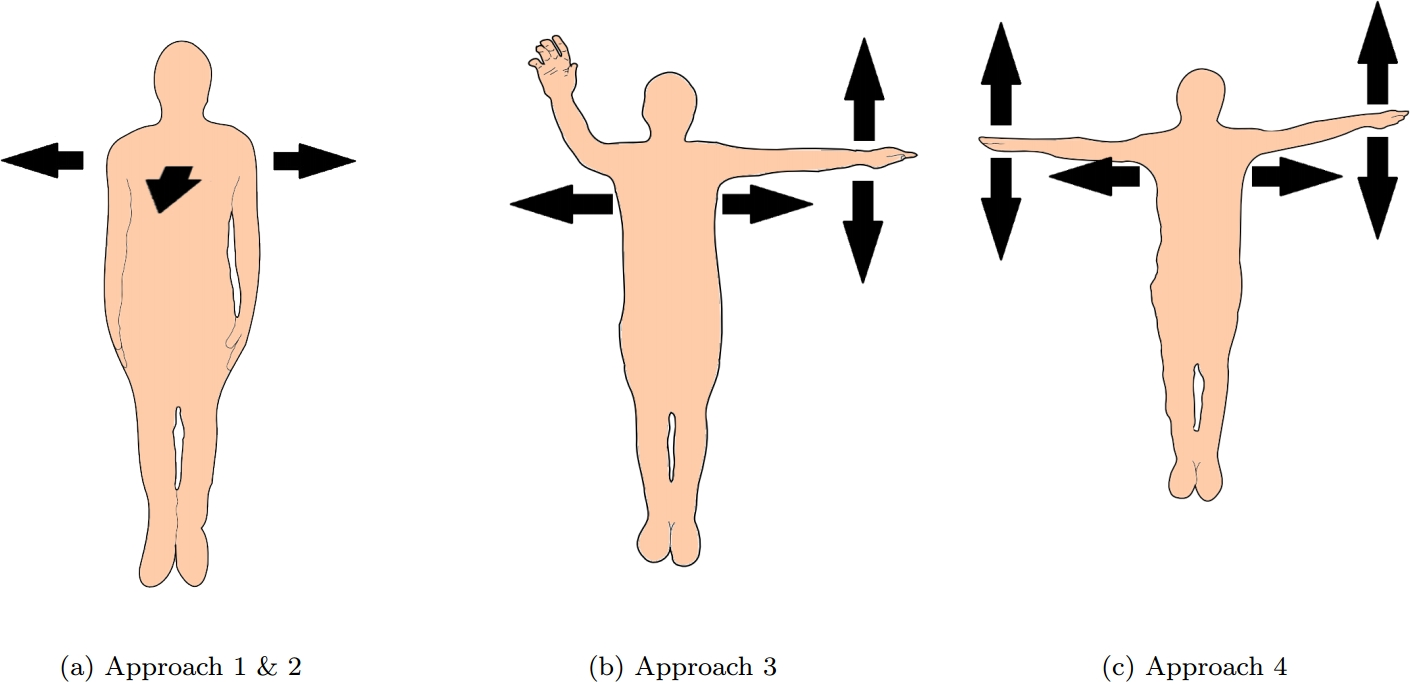
\includegraphics[width=0.5\textwidth ,keepaspectratio=true]{./img/approaches.jpg}
 \caption{Navigation approaches}
 \label{naviagationapproaches}
\end{figure}

\subsection{Selection}
Selection is needed when there is a group of enemy aircrafts. The auto-lock system will automatically lock onto a target in view. Because of this, there still needs to be an option for the user to select another visible aircraft that's not locked.

When the user wants to select another plane the user initiates the selection gesture by holding his/her right hand in front of his/her body.
The movement of the user's hand relative to the starting position will be used to select the enemy aircraft relative to the previously selected aircraft. We only consider the x and y movement, the user only controls 2 DOF (the same way as in the image-plane technique \cite{bookimageplane}).

The selected enemy aircraft will not be selected immediately but feed-forward will be given until a selection is made (a green rectangle will surround the enemy jet fighter). Once the correct enemy is selected, the user has to confirm the selection.
We first tried confirming the selection by retracting the arm, but when the user retracts his arm he often accidentally selects a different target before confirming. We solved this by letting the user press a button on a foot pedal instead of retracting his arm.

\subsection{Manipulation}
The user has the ability for manipulation by shooting enemy aircrafts. After dealing a certain amount of damage to an aircraft, it will explode. There are two kinds of weapons for the player to choose from: a machine gun and a homing missile. The machine gun will fire straight forward (Figure \ref{machinegun}).
\begin{figure}[ht]
\centering
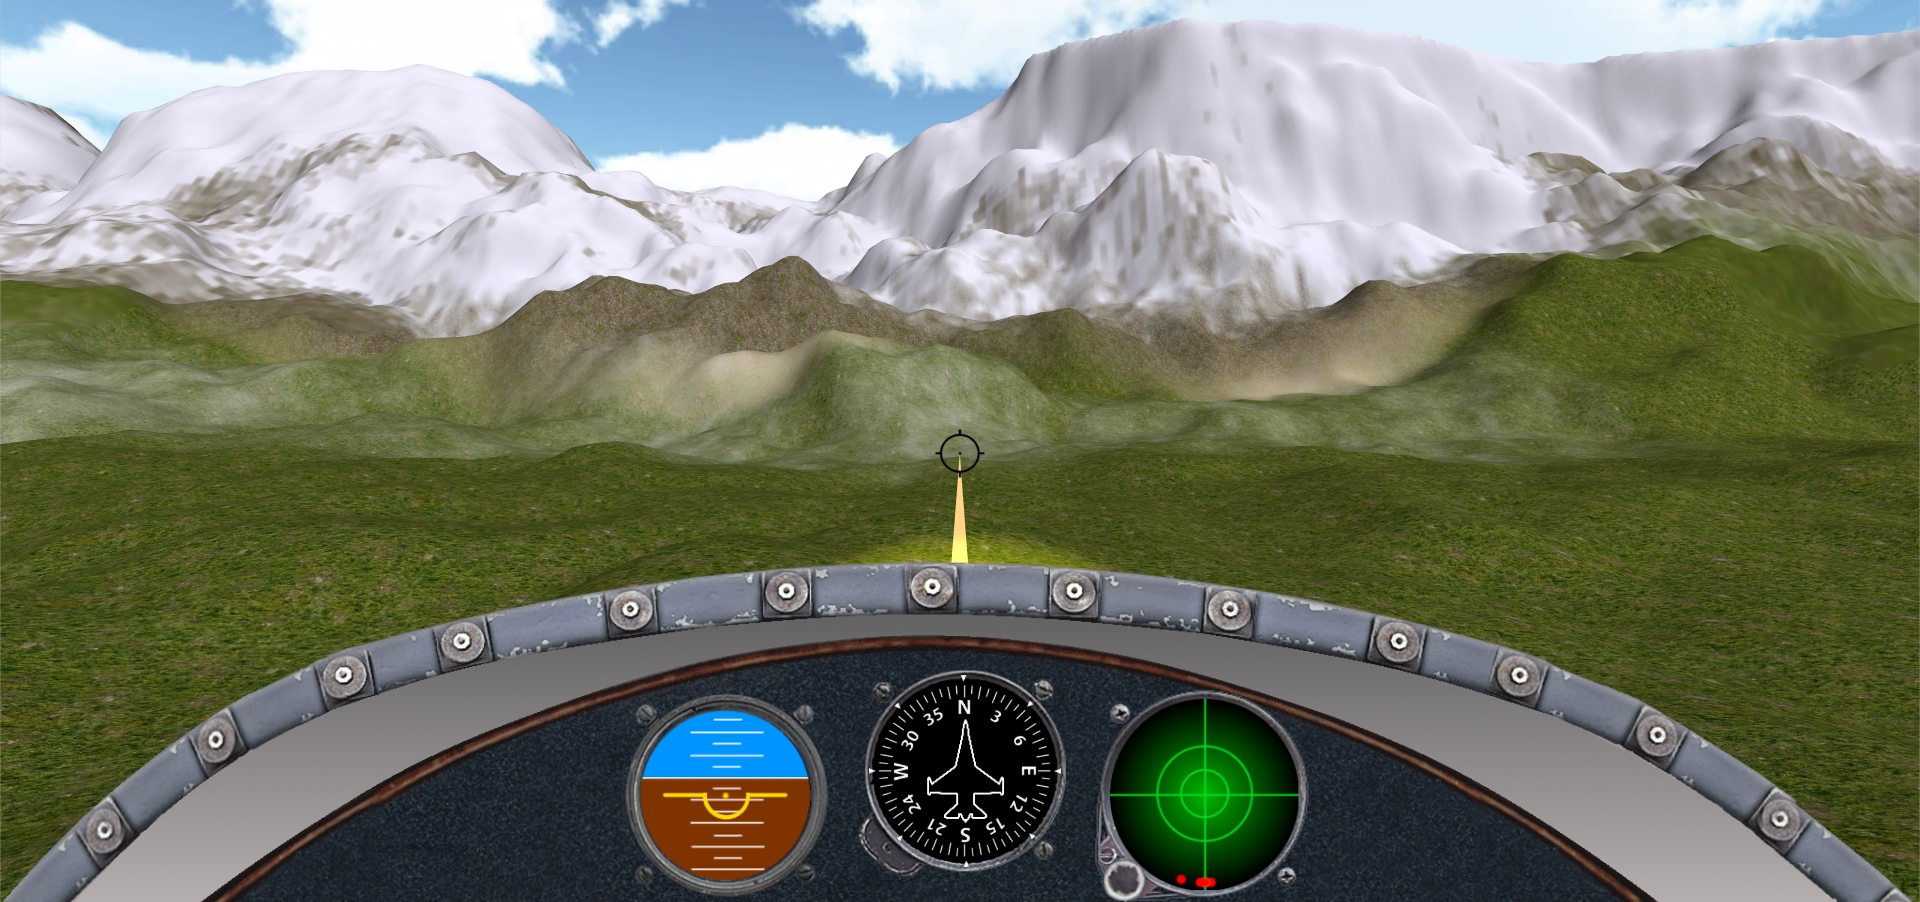
\includegraphics[width=0.5\textwidth ,keepaspectratio=true]{./img/machineGun.jpg}
 \caption{The jet fighter firing the machine gun}
 \label{machinegun}
\end{figure}

The homing missile will fly directly to the targeted enemy aircraft and follow it until it hits the aircraft (Figure \ref{missile}).
\begin{figure}[t]
\centering
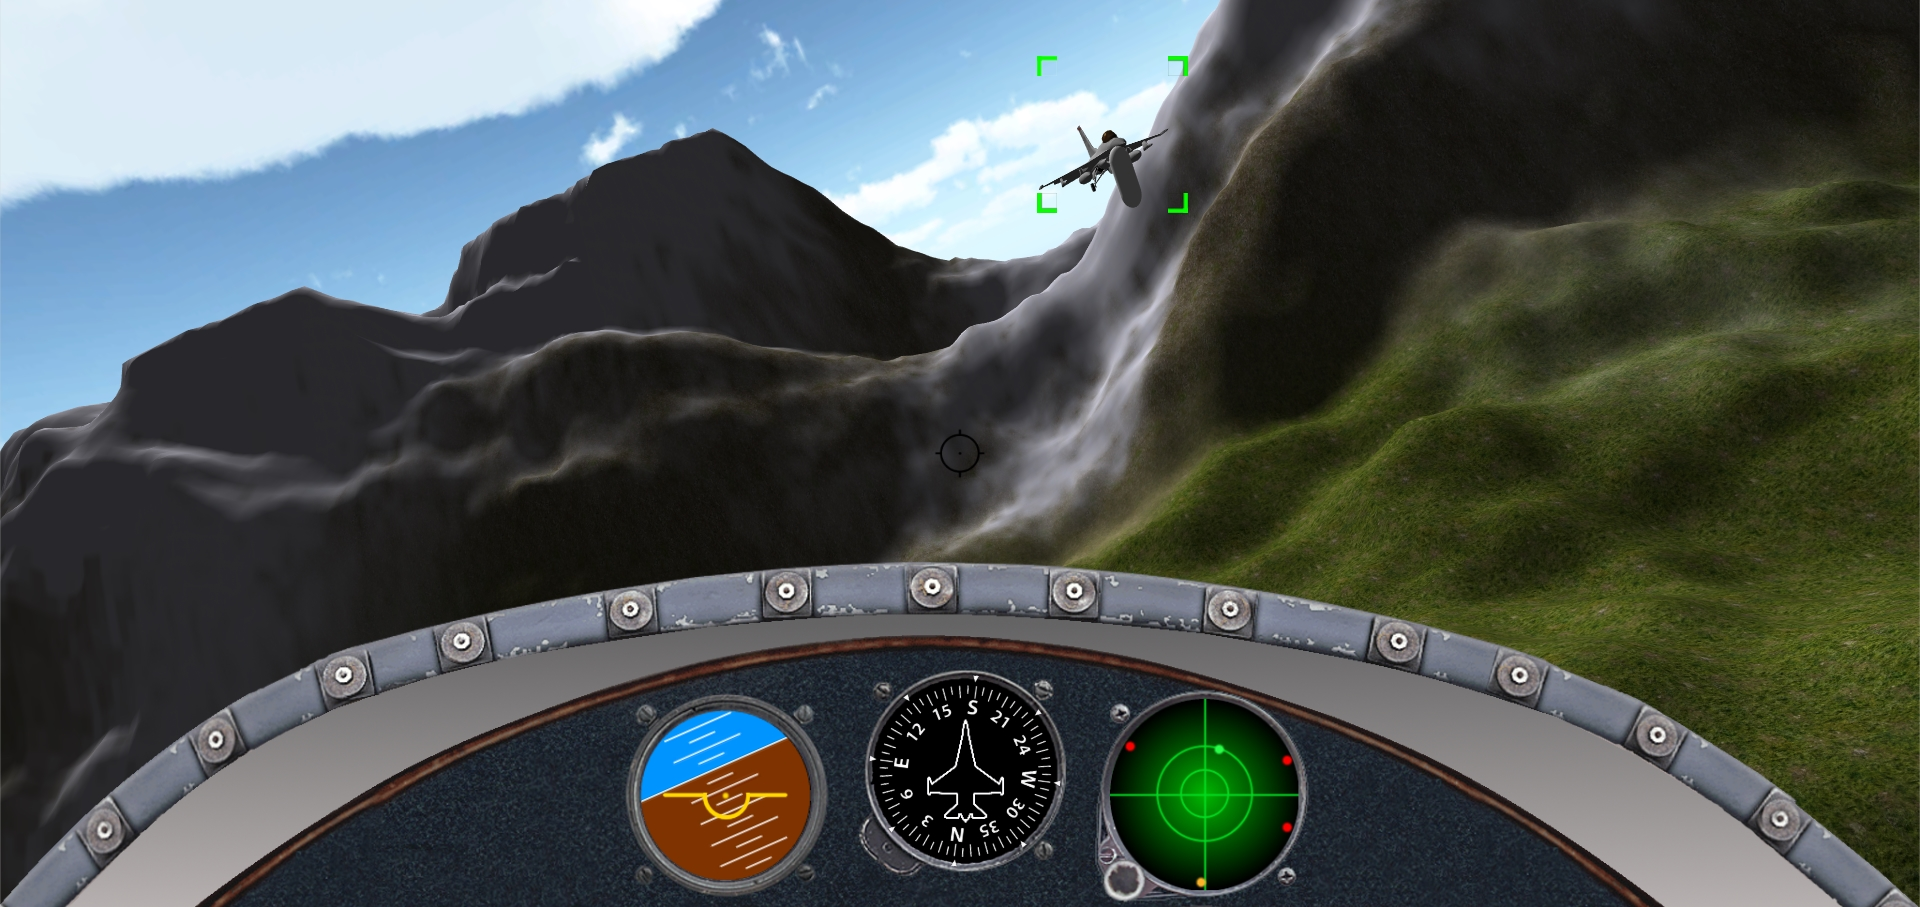
\includegraphics[width=0.5\textwidth ,keepaspectratio=true]{./img/missile.jpg}
\caption{The jet fighter firing a homing missile}
 \label{missile}
\end{figure}

\section{Dashboard}
We added a dashboard to provide the user some artificial cues to improve wayfinding. The dashboard has an attitude indicator which informs the user of the orientation of the jet relative to Earth's horizon. It also has a heading indicator (compass) and a radar which informs the user of the location of enemy planes.

\newpage


\begin{figure}[Ht]
\centering
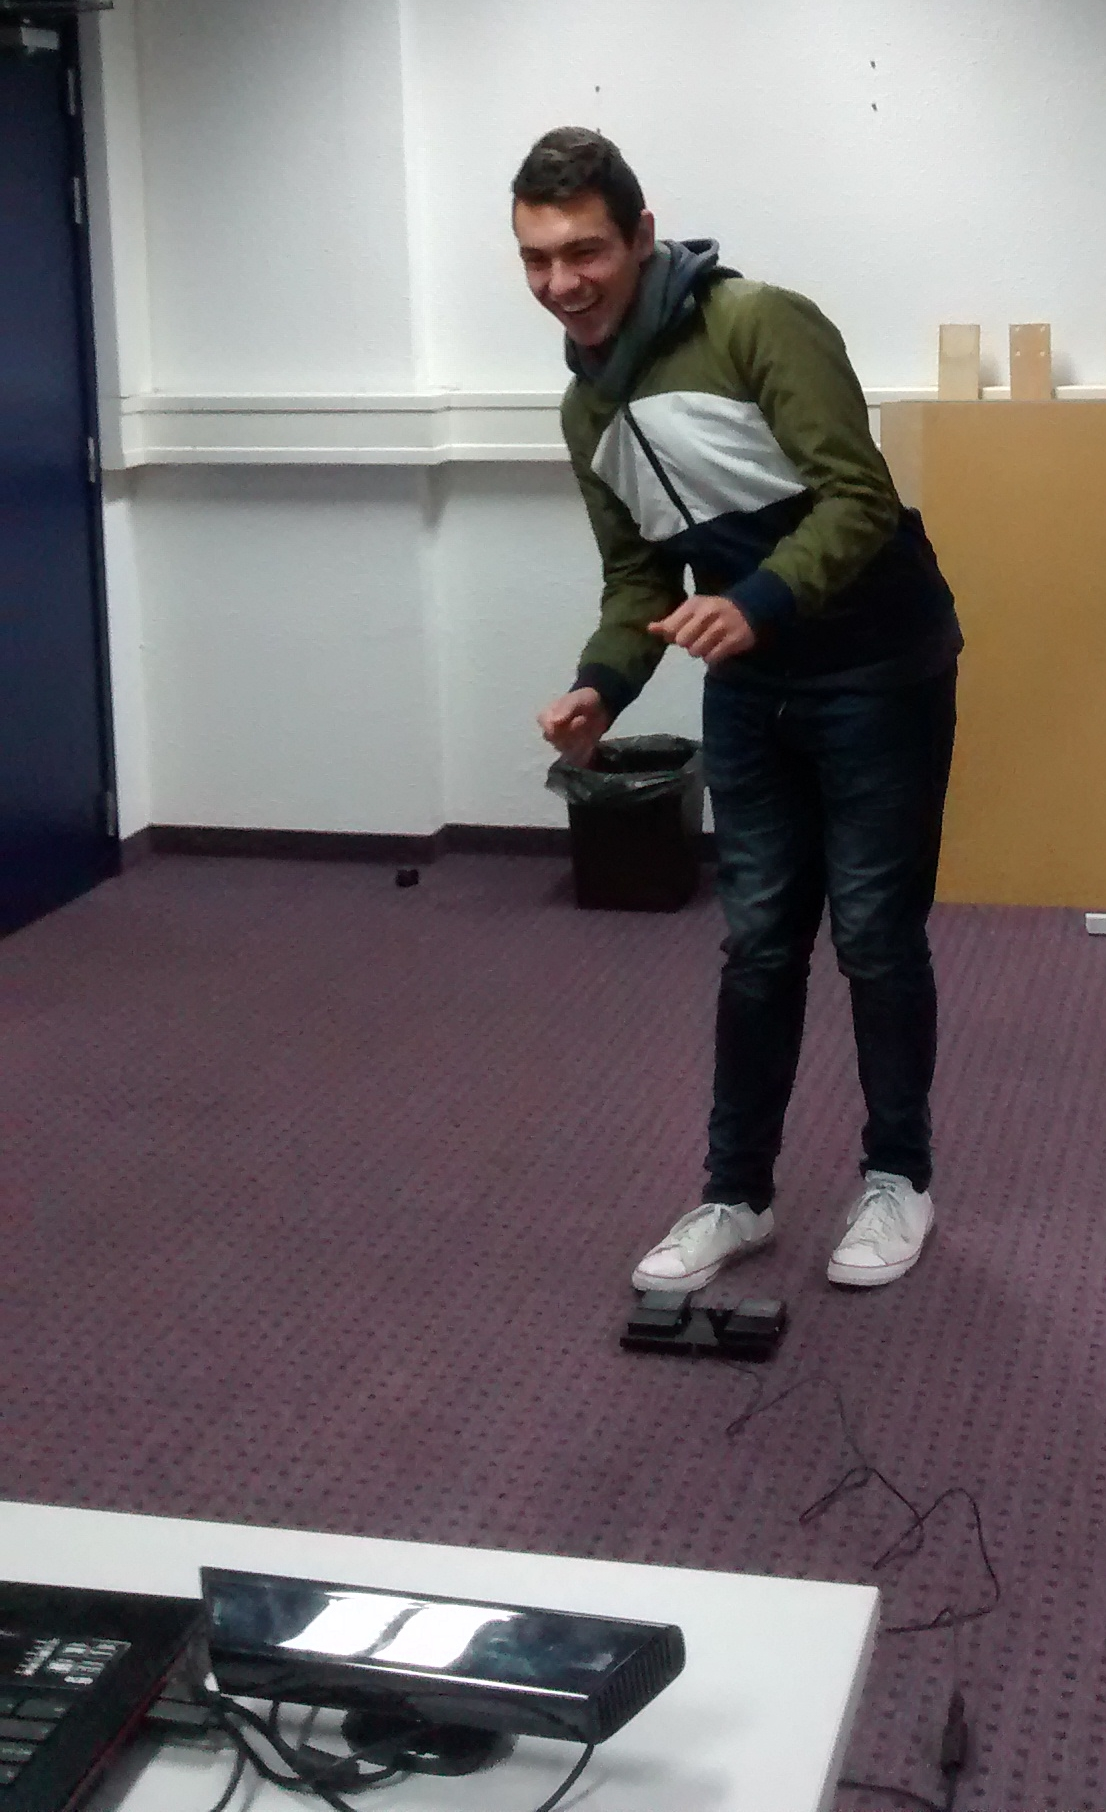
\includegraphics[width=0.3\textwidth ,keepaspectratio=true]{./img/usertest.jpg}
\caption{A user testing our application}
 \label{usertester}
\end{figure}

\section{Evaluation}
The application was tested by our fellow students in an informal usability test.
Each person tested the different aspects of the game separately and later on simultaneously.
To separate navigation from selection and manipulation, we disabled navigation to test all the other gestures independently of the navigation. This includes the navigation of the user and the navigation of the enemy jet fighter.

Firstly the users tried out the gestures for shooting with the machine gun and firing a missile.
The game selects an enemy jet fighter automatically so there is no need for the user to use a pointing gesture to select an enemy jet fighter.

Secondly the pointing and selection gestures were tested with a various numbers of targets to test how well the selection technique scaled. We tested the selection technique with 5, 20 and 50 targets.
The game selected a random enemy jet fighter randomly which the user had to select and confirm.

The third part of the test is about testing navigation, therefore we only enabled navigation and disabled selection and manipulation.
We tested the three navigation techniques separately, for each technique we followed the same steps listed below.
First the user has the opportunity get used to to navigating the jet fighter with a certain navigation technique by flying around freely.
Once the user is accommodated to the navigation technique the goal is to navigate the jet fighter through a a set of rings from start to finish following a trajectory.
There are two difficulty levels for the navigation tests, an easy one where the user only have to navigate up and down and a harder one where the user also has to turn the jet fighter left and right.

The last part of the test includes all the previously tested features of the application using navigation, selection and manipulation.
The user has to destroy the enemy jet fighters that are flying around by shooting at them using the machine gun or firing a missile after selecting them.

\subsection{Results usability test}
The shooting gestures are found easy to understand and perform by users. However sometimes users accidentally fired a missile when trying to fire the machine gun, this is not the user's fault, but a bug in gesture recognition.

There were no problems with selecting targets, all users managed to select all targets. There were also no difficulties confirming selections with the foot pedal.
The pointing selection technique scaled well from 5 to 50 targets.

Users have no problem navigating only up and down and rotating left and right. The main problem with all three navigation techniques was to move the jet fighter left and right. To achieve this users have to lean left or right while leaning backwards or forwards, which is not beneficial for the user comfort. Users expected the jet fighter to move left and right when they themselves moved left and right. This is confusing while playing the game or completing certain goals and decreases ease of use.

Most users said they preferred method 4, but one user indicated that although she preferred method 4, method 2 was the easiest for the navigation task (flying through rings).
However, we could not clearly determine which method was best for navigating based on the results from the navigation task.


There is a clear difference between what the users perceive as the most useful method and the results of the navigation task. We think the main reason for this is because users could not use the autopilot (from method 4) in the navigation task, although this is a very big part of the navigation (for method 4) in the game.

We noticed it was hard for users to recover from mistakes (e.g. after accidentally flying in the wrong direction). For example, there was one user who immediately started to fly in the wrong direction, she missed all targets and couldn't reach the finish. When we gave her a second chance, she got all targets and reached the finish.



\section{Conclusion}
Our research topic was a 3D virtual environment first-person jet fighter shooter game with Kinect navigation.
For this paper we developed four different navigation techniques to map the usable actions onto Kinect gestures. We decided that getting this many actions mapped onto a gestures can confuse the user because he/she can lose track of the different gestures. Mapping six different actions onto Kinect-gestures was tricky to find good trackable positions for them while the user would still be able to easily perform these gestures.
We also concluded that our fourth navigation technique was the best one because the auto-pilot sets the user back on a perfect track towards an enemy.

%
% The following two commands are all you need in the
% initial runs of your .tex file to
% produce the bibliography for the citations in your paper.
\nocite{*}
\bibliographystyle{acm}
\bibliography{bib}
% You must have a proper ".bib" file
%  and remember to run:
% latex bibtex latex latex
% to resolve all references
%
% ACM needs 'a single self-contained file'!
%
%APPENDICES are optional
%\balancecolumns

\balancecolumns
% That's all folks!
\end{document}
